\section{Pointer und Referenzen} 
Bei Variablenübergabe (call by value) werden Kopien übergeben, welche nicht verändert werden können.\\
Bei Referenzübergabe (call by reference) kann die Subroutine die Werte bleibend verändern. \\
\textbf{Objekte einer Klasse und Strukturvariablen sollen immer by reference übergeben werden!} \\
\subsection{call by reference}
\vspace{-13pt}
\begin{multicols}{2}
	statisch:
	\begin{lstlisting}
		void swap(int& a, int& b){
			int tmp = a;
			a = b;
			b = tmp;
		}
		int main(){
			int x = 4;
			int y = 3;
			swap(x, y);// OK!
			return 0;
		}	
	\end{lstlisting}
	dynamisch:
	\begin{lstlisting}
		void swap(int* a, int* b){
			int tmp = *a;
			*a = *b;
			*b = tmp;
		}
		int main(){
			int x = 4;
			int y = 3;
			swap(&x, &y);// OK!
			return 0;
		}
	\end{lstlisting}
\end{multicols}
\subsection{call by value}
	\begin{lstlisting}
		void swap(int a, int b){
			int tmp = a;
			a = b;
			b = tmp;
		}
		int main(){
			int x = 4;
			int y = 3;
			swap(x, y); // keine Auswirkung
			return 0;
		}	
	\end{lstlisting}
\subsection{return by reference}
\begin{lstlisting}
	int& inc(int& i){
		return ++i;
	}	
\end{lstlisting}
Der Funktionsaufruf ist nun selbst ein L-Wert, was nun Ausdrücke wie \texttt{inc(inc(x))} oder \texttt{++inc(x)} erlaubt. \textbf{Achtung} Gültigkeitsbereiche: Return by reference auf lokale Variable ist undefined behavior.
\subsection{Pointer}
Ein Ausdruck vom Typ \texttt{T*} heisst Zeiger (Auf T). Der Wert eines Zeigers ist die Adresse, auf die er zeigt. Man kommt auf die Adresse eines Objektes entweder direkt beim Erzeugen mittels \texttt{new} oder mit dem Adress-Operator \texttt{\&}.Um undefiniertes Verhalten bei der Initialisierung zu vermeinden, erstellt man einen Null-Zeiger.
\begin{lstlisting}
	int* r; //undefined behaviour
	int* q=nullptr; //(zeigt explizit ins nichts)
	
	int i = 5;
	int* p = &i; //Zeiger auf i
	std::cout<<*p; // Output: 5
\end{lstlisting}
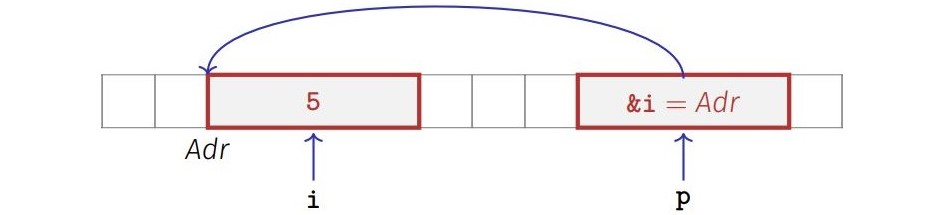
\includegraphics[width=0.24 \textwidth]{sections/pointer}
Um nun der Wert bei der Adresse des Pointers zu erhalten braucht man den Deferenz-Operator \texttt{*}.
\subsubsection{Pointerarithmetik}
Mit Pointer kann gerechnet werden.
\begin{lstlisting}
	int* p0 = new int[7]{1,2,3,4,5,6,7};
	int* p3 = p0 + 3; //p3 zeigt auf das 4.te Element
	++p0 // p0 zeigt neu auf das 2.te Element.
\end{lstlisting}
Speicher der mit \texttt{new Typ} alloziert wurde, wid nicht automatisch freigegeben. Mit Pointer kann mann auch wahlfreien Zugriff auf Arrays machen. \texttt{*(p0 + i)} ist das selbe wie \texttt{p[i]}. Die übergabe eines Arrays erfolgt oft mittels zwei Zeigern \texttt{begin} (erstes Element) und \texttt{end} (hinter letztes Element)
Wenn Werte von Zeigern, oder Zeiger selber nicht verändert werden soltlen, kann diese Garantie mit \texttt{const} gegeben werden. Man liest die Deklaration von rechts nach links.
\begin{lstlisting}
	int const p1; //konst. Wert
	int const* p2 //Zeiger auf konst. Wert
	int* const p3; // konst. Zeiger auf Wert
	int const* const p4; //konst. Zeiger auf konst. Wert
	
\end{lstlisting}




